\documentclass[]{article}
\usepackage{graphicx}
\newtheorem{Def}{Definition}

%opening
\title{MTH 343 Numerical Analysis Lecture 3: Errors, Solutions of Equations in one Variable}
\author{Sheikh Abdul Raheem Ali}

\begin{document}

\maketitle

The floating point form is obtained by terminating the mantissa using the following two ways:

\begin{enumerate}
	\item Chopping
	\item Rounding
\end{enumerate}

\begin{Def}[Absolute error]
$	|true \ value - approximate \ value| = |p - p^*| $
\end{Def}

\begin{Def}[Relative error]
$ |\frac{true \ value \ - \ approximate \ value}{true \ value}| =  |\frac{p \ - \ p^*}{p}| $
\end{Def}

\[  (approximate \ value ) \ p_1 = 1.2, \ (true \ value) \ p_1^* = 1.2 \]
\[  p_2 = 1000, \ p_2^* = 1000.2 \]

\begin{eqnarray}
absolute \ error &=&  |1 - 1.2| = 0.2 \nonumber \\
&=& |1000 - 1000.2| = 0.2 \nonumber
\end{eqnarray}

\begin{eqnarray}
	rel. \ error &=& |\frac{1 - 1.2}{1}| = 0.2 \nonumber \\
	&=&  |\frac{1000 - 1000.2}{1000}| = 0.0002 \nonumber 
\end{eqnarray}

\[ find \ f(x) = x^3 = 61x^3 + 3.2x + 1.5 \ at \ f(x = 4.71) \]

\begin{tabular}{l c c c c c}
	& $ x $ & $ x^2 $ & $ x^3 $ & $ 61x^3 $ & $ 3.2x $ \\ \hline
	Exact &4.7&22.1841&104.487111&135.32301&15.072\\
	3-digit chopping &4.7&22.1&104.0&134&15.0 \\
	3-digit rounding &4.7&22.2&104&135&15.1 \\
	
\end{tabular}

Exact: -14.263899, Chopping: -13.5. Rounding: -13.4 \\
Rel. error: Chopping: 0.0045, Rounding: 0.0025

\section*{Solutions of Equations of one variable}

\begin{eqnarray}
	0 &=& x^3 - 16x \nonumber \\
	&=& x(x^2 - 16) \nonumber\\
	&=& x(x-4)(x+4) \nonumber\\
	 x = 0,4,-4 \nonumber
\end{eqnarray}

\begin{eqnarray}
	0 &=&  x^2 - 4x + 3x - 12 \nonumber \\ 
	&=& x(x-4) + 3(x-4) \nonumber \\
	&=& (x-4)(x-3) \nonumber \\
	x = 4,3 \nonumber
\end{eqnarray}

\section*{Bisection Method (f(x) = 0)}

Find the values of $ x $ for which $ f(x) = 0, $ that is find the points of intersection of $ f(x) $ with the x-axis. 

\begin{figure}
	\centering
	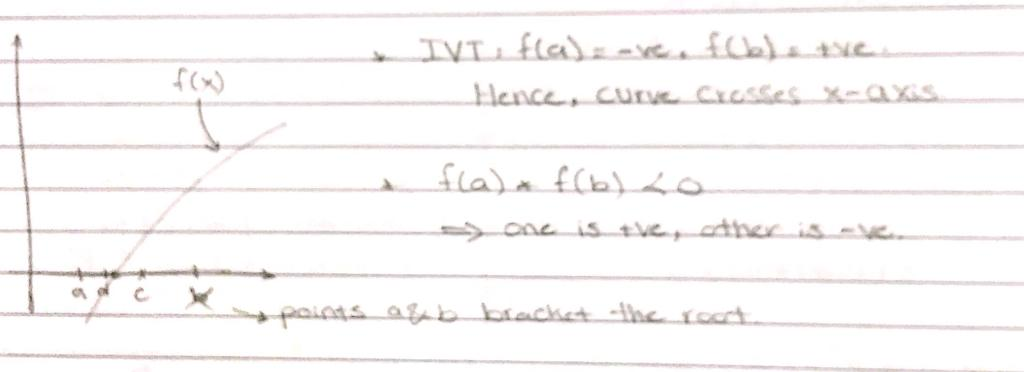
\includegraphics[width=\linewidth]{graph.jpeg}
	\caption{Visual demonstration of the bisection algorithm. Credits to Luna Hatahet. }
	\label{fig:graph}
\end{figure}


\end{document}
